\documentclass{research4cacm}

%%% Note to copy editors: the following fixes are needed
%%% in order to get decent output in the temporary version
%%% for the submission
\makeatletter
\renewcommand{\secfnt}{\fontfamily{ptm}\fontsize{12}{14}\bfseries}
\renewcommand{\subsecfnt}{\fontfamily{ptm}\fontsize{11}{13}\itshape}
\def\section{%
    \@startsection{section}{1}{\z@}{-10\p@ \@plus -4\p@ \@minus -2\p@}% GM
    {14\p@}{\secfnt\@ucheadtrue}%
}

\def\subsection{%
    \@startsection{subsection}{2}{\z@}{-8\p@ \@plus -2\p@ \@minus -\p@}
    {14\p@}{\secfnt}%
}
\def\subsubsection{%
    \@startsection{subsubsection}{3}{\z@}{-8\p@ \@plus -2\p@ \@minus -\p@}%
    {14\p@}{\subsecfnt}%
}
\expandafter\def\expandafter\abstract\expandafter{\abstract\vspace{-\baselineskip}}
\makeatother
%%% end of fixes

%\usepackage[T1]{fontenc}
%\usepackage{lmodern}
%\usepackage[a-2b]{pdfx}
%\usepackage{amsmath}
%\usepackage{amsfonts}
%%\usepackage[utf8]{inputenc}
\usepackage{array}
%\usepackage{stmaryrd}
\usepackage{tikz}
\usepackage{comment}
\usepackage{xspace}
\usepackage{listofitems}
%\usepackage{graphicx}
\usepackage[final]{listings}
%\usepackage{enumitem}
%%\usepackage{amsthm}
\usepackage{ifthen}
\usepackage{url}

% space saving tricks
\newif\ifstreamexamples
\streamexamplestrue
\newif\ifzsetexamples
\zsetexamplestrue
%%\newtheoremstyle{note} % name
%%{2pt} % Space above
%%{2pt} % Space below
%%{}    % Body font
%%{}    % Indent amount
%%{\bfseries} % Theorem head font
%%{:}   % Punctuation after theorem head
%%{.5em}% ⟨Space after theorem head
%%{}    % Theorem head spec (can be left empty, meaning ‘normal’
%
%\numberwithin{equation}{section}
%
%\graphicspath{ {.} }
\lstset{language=Java,
  commentstyle=\color{brown},
  keywordstyle=\color{blue},
  stringstyle=\color{red},
  basicstyle=\ttfamily}

\lstdefinelanguage{ddlog}{
  language=Java, % we base it on Java, just for comments
  morekeywords={input, output, typedef, relation, typedef, bool, not,
    string, bit, extern, function, var, for, match, skip, in, integer, % not really in DDlog
    Aggregate, FlatMap},
  deletestring=[b]{'}
}
%\hypersetup{
%  colorlinks   = true,    % Colours links instead of ugly boxes
%  urlcolor     = blue,    % Colour for external hyperlinks
%  linkcolor    = blue,    % Colour of internal links
%  citecolor    = red      % Colour of citations
%}
%\hypersetup{final}
%
\usetikzlibrary{shapes, arrows.meta, positioning}
\tikzstyle{block}=[draw,fill=white,rectangle]
\tikzstyle{every node}=[font=\small]

%\theoremstyle{note}
\newtheorem{theorem}{Theorem}[section]
\newtheorem{lemma}[theorem]{Lemma}
\newtheorem{corollary}[theorem]{Corollary}
\newtheorem{definition}[theorem]{Definition}
\newtheorem{proposition}[theorem]{Proposition}
\newtheorem{example}[theorem]{Example}
\newtheorem{algorithm}[theorem]{Algorithm}

\begin{document}

% Used when a term is first defined.  Adds the term to the index.
\newcommand{\defined}[1]{\textbf{#1}\index{}}
\newcommand{\zr}{$\Z$-set\xspace}
\newcommand{\zrs}{$\Z$-sets\xspace} % plural
\newcommand{\means}[1]{\ensuremath{\llbracket #1 \rrbracket}}
\newcommand{\code}[1]{\mbox{\texttt{#1}}}
\newcommand{\Z}{\mathbb{Z}}  % integers
\newcommand{\N}{\mathbb{N}}  % naturals
\newcommand{\B}{\mathbb{B}}  % Booleans
\newcommand{\R}{\mathbb{R}}  % reals
% stream with elements of a given type
\newcommand{\stream}[1]{\ensuremath{\mathcal{S}_{#1}}}
% finite stream with elements of a given type (zero almost everywhere)
\newcommand{\streamf}[1]{\ensuremath{\overline{\mathcal{S}_{#1}}}}
\newcommand{\zm}{\ensuremath{z^{-1}}} % stream delay operator
\ifthenelse{\equal{1}{1}}{ % allows switching to mathit/mathcal
\newcommand{\I}{\mathcal{I}}  % stream integration
\newcommand{\D}{\mathcal{D}}  % stream derivative
}{
\newcommand{\I}{\mathit{I}}  % stream integration
\newcommand{\D}{\mathit{D}}  % stream derivative
}
\newcommand{\inc}[1]{{#1}^{\Delta}}
\newcommand{\distinct}{\mathit{distinct}}  % distinct operator
% set with elements of given type
\newcommand{\secref}[1]{\S\ref{#1}}  % reference to a section
\newcommand{\refsec}[1]{\secref{#1}}
\newcommand{\set}[1]{\mathit{set}_{#1}}
\newcommand{\id}{\ensuremath{\mathit{id}}} % identity function
\newcommand{\isset}{\mbox{isset}}
\newcommand{\ispositive}{\mbox{ispositive}}
\newcommand{\defn}{\stackrel{\textrm{\scriptsize def}}{=}}
\newcommand{\map}{\mbox{map}}
\newcommand{\fix}[2]{\mbox{fix}\,#1.#2}
\newcommand{\lift}[1]{{\uparrow}#1}
\newcommand{\rew}{\ensuremath{\mapsto}} % rewriting
\newcommand{\birew}{\ensuremath{\mapsfrom\!\mapsto}} % bidirectional rewriting
\newcommand{\pair}[2]{\ensuremath{\langle #1,#2 \rangle}} % pairing
\newcommand{\norm}[1]{\| #1 \|} % norm; requires math mode
%\newcommand{\zpp}[1]{\mbox{zpp}(#1)}
\newcommand{\makeset}{\ensuremath{\mbox{makeset}}}
\newcommand{\sv}[1]{ % simple stream value, supplied as a space-separated list of 5 values
\setsepchar{ }
\readlist\arg{#1}
{[}
\begin{array}{cccccc}
    \arg[1] & \arg[2] & \arg[3] & \arg[4] & \arg[5] & \cdots
\end{array}
{]}
}

\newcommand{\dbsp}{DBSP\xspace}
\numberofauthors{5}
\author{
  \alignauthor Mihai Budiu \\
  \affaddr{Feldera} \\
  \email{mbudiu@feldera.com} \\
  \alignauthor Tej Chajed \\
  \affaddr{University of Wisconsin-Madison} \\
  \email{chajed@wisc.edu} \\
  \alignauthor Frank McSherry \\
  \affaddr{Materialize Inc.} \\
  \email{mcsherry@materialize.com} \\
  \and
  \alignauthor Leonid Ryzhyk \\
  \affaddr{Feldera} \\
  \email{ryzhyk@feldera.com} \\
  \alignauthor Val Tannen \\
  \affaddr{University of Pennsylvania} \\
  \email{val@seas.upenn.edu} \\
}

\title{\dbsp: Automatic Incremental View Maintenance for Rich Query Languages}
\maketitle

\begin{abstract}
Incremental view maintenance (IVM) has long been a central problem in
database theory.  Many solutions have been proposed for restricted
classes of database languages, such as the relational algebra, or
Datalog.  These techniques do not naturally generalize to richer
languages.  In this paper we give a general, heuristic-free solution
to this problem in 3 steps: (1) we describe a simple but expressive
language called \dbsp for describing computations over data streams;
(2) we give a new mathematical definition of IVM and a general
algorithm for solving IVM for arbitrary \dbsp programs, and (3) we
show how to model many rich database query languages using \dbsp
(including the full relational algebra, queries over sets and
multisets, arbitrarily nested relations, aggregation, flatmap
(unnest), monotonic and non-monotonic recursion, streaming
aggregation, and arbitrary compositions of all of these).  SQL and
Datalog can both be implemented in \dbsp.  As a consequence, we
obtain efficient incremental view maintenance algorithms for queries
written in all these languages.
\end{abstract}

\permission{}
\copyrightetc{Copyright is held by the owner/author(s). Publication
  rights licensed to the VLDB Endowment. This is a minor revision of
  the paper entitled \dbsp: Automatic Incremental View Maintenance for
  Rich Query Languages, published in PVLDB, Vol. 16, Issue 7, ISSN
  2150-8097.  DOI: https://doi.org/10.14778/3587136.3587137}

\section{Introduction}\label{sec:introduction}

This paper is an extended version of a VLDB 2023
publication~\cite{budiu-vldb23}, adopting the notations
from~\cite{budiu-sigmod24}.  The major changes are: adding new
incremental program examples (\refsec{sec:recursive-example},
\refsec{sec:recursive-incremental-example}), an expanded discussion of
implementing SQL with its ``standard'' semantics~\refsec{sec:sql}, an
extended implementation section~\refsec{sec:implementation}, and a
preliminary experimental evaluation~\refsec{sec:experiments}.  This
paper includes only a few short mathematical proofs; all the proofs
can be found in an extended technical report~\cite{tr}; the proofs
have also been formalized and verified in the Lean proof
assistant~\cite{dbsp-theory}.

\subsection{Problem and Solution Overview}\label{sec:intro-incremental}

The IVM problem can be stated as follows: we are given a database $DB$
and a view $V$, described by a query $Q$.  The goal of IVM is to keep
the contents of $V$ up-to-date in response to changes of the database.

Consider the following SQL statement:

\begin{lstlisting}[language=SQL]
CREATE VIEW V AS
SELECT * FROM T WHERE Age >= 10
\end{lstlisting}

In this example the query $Q$ defining the view $V$ is the
\code{SELECT} statement.  The view \code{V} always contains all the
rows of table \code{T} whose value for the column \code{Age} is
greater than or equal to 10.

In general a query is a function applied to the contents of a
database: $V = Q(DB)$.  A naive solution re-executes query $Q$ every
time the database changes, as illustrated in the following diagram.
Time is the horizontal axis; the horizontal arrows labeled with
$\Delta$ depict changes to the database.  The ``up'' arrows show the
re-evaluation of $Q$ for each database snapshot.

\noindent \includegraphics[trim={0 4.8in 3.7in 0},clip,scale=.34]{view.pdf}

The naive solution is expensive.  An ideal algorithm would compute
only \emph{changes} to the view $\Delta V$, doing work $O(|\Delta DB|)$
(after computing the first version of the view).

\noindent \includegraphics[trim={0 5.2in 4.1in 0},clip,scale=.35]{incview.pdf}

We call $\inc{Q}$ the \emph{incremental} version of $Q$.  For an
arbitrary query $Q$ one can show that there is no solution where
$\inc{Q}$ is a (pure) function of $\Delta DB$ (only restricted classes
of queries have such solutions).

In this paper we propose a new way to define $\inc{Q}$, as a form of
\emph{computation on streams}.  Our model is inspired by Digital
Signal Processing DSP~\cite{rabiner-book75}, applied to databases,
hence the name \dbsp.

$\inc{Q}$ can be significantly more efficient than the naive
solution.  As is the case for traditional database queries, the
performance of $\inc{Q}$ depends both on the query $Q$ but also on the
actual data that the query is applied to.  Informally, $\inc{Q}$ built
by our algorithm, is faster than $Q$ by a factor of $O(|DB| / |\Delta
DB|)$.  In practice this may be an improvement of several orders of
magnitude.

Instead of treating the database as a large, changing object, we model
it as a sequence or \emph{stream} of database snapshots, shown as
$DB[1], DB[2], \ldots$ in the previous diagrams.  Similarly,
consecutive view snapshots form a stream.  \dbsp is a simple
programming language computing on streams; inputs and outputs are
streams of arbitrary values.

The \dbsp language has only 4 operators.  However, it can express a
rich set of computations on streams, including repeated computations
(similar to the repeated queries $Q$ above), recursive computations
that compute fixed points (like Datalog programs), more general
streaming computations, and incremental computations (defined
shortly).

The central result of this paper is Algorithm~\ref{algorithm-inc}
in~\refsec{sec:relational}.  The input to the algorithm is a \dbsp
program that computes on a stream of data; the algorithm mechanically
transforms it into an incremental \dbsp program that computes on a
stream of changes.

\dbsp is not tied to databases in any way; it is in fact a
Turing-complete language that can be used for many other purposes.
But it works particularly well in the area of databases, for two
reasons:

\begin{itemize}[nosep, leftmargin=0pt, itemindent=0.5cm]
  \item \dbsp operates on values from a commutative group.  Databases
    can be modeled as a commutative group.
  \item \dbsp reduces the problem of incrementalizing a complex
    program to the problem of incrementalizing each primitive
    operation that appears in the program.  For databases there are
    known efficient incremental implementations for all primitive
    operations.
\end{itemize}

\subsection{Core abstractions}

\subsubsection{Circuits}

In this paper we use circuit diagrams to depict programs.  In a
circuit a rectangle represents a function, and an arrow represents an
input or output value.  The following diagram shows a function $f$
consuming two inputs $i$ (input 0) and $j$ (input 1) and producing one
output $o = f(i, j)$:
%
\begin{center}
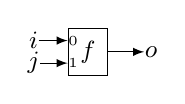
\begin{tikzpicture}[auto,>=latex,inner sep=0mm]
  \node[block, minimum height=.6cm, minimum width=.5cm] (function) {$f$};
  \node[below=1mm of function.north west,font=\tiny,anchor=north west] (0) {0};
  \node[above=1mm of function.south west,font=\tiny,anchor=south west] (1) {1};
  \node[left of=0, node distance=.5cm] (input0) {$i$};
  \node[left of=1, node distance=.5cm] (input1) {$j$};
  \node[right of=function, node distance=.8cm] (output) {$o$};
  \draw[->] (input0) -- (0);
  \draw[->] (input1) -- (1);
  \draw[->] (function) -- (output);
\end{tikzpicture}
\end{center}

%
Most of the functions we deal with are commutative, so we omit input
labels, showing the circuit above as:
%
\begin{center}
  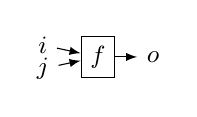
\begin{tikzpicture}[auto,>=latex, node distance=.7cm]
    \node[] (input0) {$i$};
    \node[below of=input0,node distance=.15cm] (dummy) {};
    \node[below of=dummy,node distance=.15cm] (input1) {$j$};
    \node[block, right of=dummy] (T) {$f$};
    \node[right of=T] (output) {$o$};
    \draw[->] (input0) -- (T);
    \draw[->] (input1) -- (T);
    \draw[->] (T) -- (output);
  \end{tikzpicture}
\end{center}

%
Functions, and their circuits, can be composed, as in the following
example showing $o = g(s) + (f(s) \times s)$:
%
\begin{center}
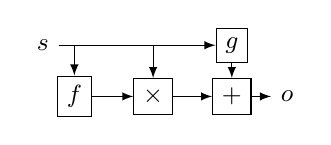
\begin{tikzpicture}[auto,>=latex]
  \node[] (input) {$s$};
  \node[] [right of=input, node distance=.4cm] (dummy) {};
  \node[block, below of=dummy, node distance=.65cm] (S1) {$f$};
  \node[block, right of=S1] (T1) {$\times$};
  \node[block, right of=T1] (T2) {$+$};
  \node[block, above of=T2, node distance=.65cm] (S2) {$g$};
  \node[right of=T2, node distance=.7cm] (output) {$o$};
  \draw[->] (input) -| (S1);
  \draw[->] (input) -| (T1);
  \draw[->] (S1) -- (T1);
  \draw[->] (T1) -- (T2);
  \draw[->] (input) -- (S2);
  \draw[->] (T2) -- (output);
  \draw[->] (S2) -- (T2);
\end{tikzpicture}
\end{center}

\subsubsection{Streams}

The core notion of \dbsp is the \textbf{stream}.  Given a set $A$, a
\defined{stream} \emph{of values from $A$} is an infinite sequence of
values from $A$.  $\stream{A}$ denotes the set of all streams with
values from $A$.  We write $s[t]$ for the $t$-th element of the stream
$s$.  Think of $t$ as the ``time'' and of $s[t]\in A$ as the value of
the stream $s$ ``at time'' $t$.  We show streams as a sequence of
boxes, with time from \emph{right to left}: e.g., the stream $id[t]
\defn t$ is:
%
\begin{center}
\begin{tabular}{cc}
  \sv{0 1 2 3 4} \\
  $\xleftarrow[\hspace{1cm}\mathrm{time}\hspace{1cm}]{}$
\end{tabular}
\end{center}

A \defined{stream operator} is a function that computes on streams and
produces streams.  We use ``operator'' for streams, and ``function''
for computations on ``scalar'' values.  In circuits we use arrows with
a double head to depict streams.  The following diagram shows a stream
operator $T$ consuming two input streams $s_0$ and $s_1$, producing
one output stream $s$; the difference from the previous figure is in
the use of double arrows.
%
\begin{center}
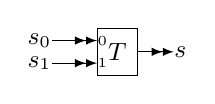
\begin{tikzpicture}[auto,>=latex,inner sep=0mm]
  \node[block, minimum height=.6cm, minimum width=.5cm] (function) {$T$};
  \node[below=1mm of function.north west,font=\tiny,anchor=north west] (0) {0};
  \node[above=1mm of function.south west,font=\tiny,anchor=south west] (1) {1};
  \node[left of=0, node distance=0.8cm] (input0) {$s_0$};
  \node[left of=1, node distance=0.8cm] (input1) {$s_1$};
  \node[right of=function, node distance=.8cm] (output) {$s$};
  \draw[->>] (input0) -- (0);
  \draw[->>] (input1) -- (1);
  \draw[->>] (function) -- (output);
\end{tikzpicture}
\end{center}
%
We write $s = T(s_0, s_1)$.

Given a function $f: A \to B$, we define a stream operator $\lift{f}
:\stream{A} \to \stream{B}$ (read as ``$f$ lifted'') by applying
function $f$ to each input value independently:

\noindent
\begin{center}
  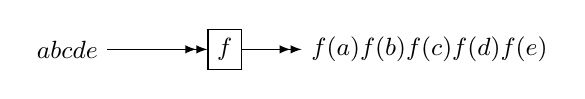
\begin{tikzpicture}[auto,>=latex]
    \node[] (input) {$\sv{a b c d e}$};
    \node[block, right of=input, node distance=2cm] (f) {$\lift{f}$};
    \node[right of=f, node distance=2.6cm] (output) {$\sv{f(a) f(b) f(c) f(d) f(e)}$};
    \draw[->>] (input) -- (f);
    \draw[->>] (f) -- (output);
  \end{tikzpicture}
\end{center}

\vspace{-3ex}

\subsection{Databases as streams}

We generally think of streams as sequences of ``small'' values, such
as insertions or deletions in a database.  However, we also treat the
whole database as a \emph{stream of database snapshots}.  We model a
database as a stream $DB$.  Time is not wall-clock time, but counts
the transactions executed.  Since transactions are linearizable, they
have a total order.  $DB[t]$ is the snapshot of the database contents
after $t$ transactions have been applied.  We use this notation in the
diagrams in \refsec{sec:intro-incremental}.

Database transactions also form a stream $\Delta DB$, which is a
stream of \emph{changes}, or \emph{deltas}, that are applied to the
database.  The values of this stream are defined by $(\Delta DB)[t] =
DB[t] - DB[t-1]$, where ``$-$'' stands for the difference between two
databases, a notion that we will soon make more precise.  The $\Delta
DB$ stream can be produced from the $DB$ stream by the \emph{stream
differentiation} operator $\D$; this operator produces as its output
the stream of changes from its input stream; we have thus $\D(DB) =
\Delta DB$.

Conversely, the database snapshot at time $t$ is the cumulative result
of applying all transactions up to $t$: $DB[t] = \Delta DB[0] + \Delta
DB[1] + \ldots + \Delta DB[t]$.  The stream operator $\I$ is defined
to produce each output by adding up all previous inputs.  We call $\I$
\emph{stream integration}, the inverse of differentiation.  The
following diagram shows the relationship between the streams $\Delta
DB$ and $DB$:
\begin{center}
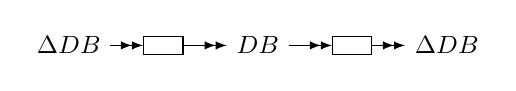
\begin{tikzpicture}[auto,>=latex,minimum width=.5cm, node distance=1.2cm]
  \node[] (input) {$\Delta DB$};
  \node[block, right of=input] (I) {$\I$};
  \node[right of=I] (output) {$DB$};
  \node[block, right of=output] (D) {$\D$};
  \node[right of=D] (end) {$\Delta DB$};
  \draw[->>] (input) -- (I);
  \draw[->>] (I) -- (output);
  \draw[->>] (output) -- (D);
  \draw[->>] (D) -- (end);
\end{tikzpicture}
\end{center}

In this model a database view is also a stream.  Suppose query $Q$
defining a view $V$.  For each snapshot of the database stream we have
a snapshot of the view: $V[t] = Q(DB[t])$.  A view is thus just a
lifted query: $V = (\lift{Q})(DB)$.

Armed with these basic definitions, we can precisely define IVM.  A
maintenance algorithm computes the \emph{changes} to the view given
the changes to the database. Given a query $Q$, a key contribution of
this paper is the definition of its \emph{incremental version}
$\inc{Q}$, using stream integration and differentiation, depicted
graphically as:

%
\begin{center}
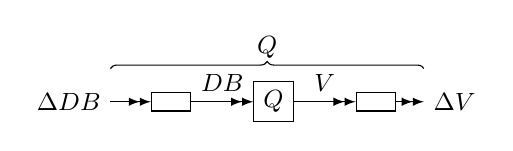
\begin{tikzpicture}[auto,>=latex,minimum width=.5cm]
  \node[] (input) {$\Delta DB$};
  \node[block, right of=input, node distance=1.3cm] (I) {$\I$};
  \node[block, right of=I, node distance=1.3cm] (Q) {$\lift{Q}$};
  \node[block, right of=Q, node distance=1.3cm] (D) {$\D$};
  \node[right of=D] (output) {$\Delta V$};
  \draw[->>] (input) -- (I);
  \draw[->>] (I) -- node (db) {$DB$} (Q);
  \draw[->>] (Q) -- node (B) {$V$} (D);
  \draw[->>] (D) -- (output);
  \draw[decorate, decoration = {brace, raise=12pt}] (input) -- (output)
  node[pos=.5, above=12pt]{$\inc{Q}$};
\end{tikzpicture}
\end{center}

%
Mathematically: $\inc{Q} = \D \circ (\lift{Q}) \circ \I$.  The
incremental version of a query $Q$ is a \emph{streaming operator}
$\inc{Q}$ which computes directly on changes and produces changes.
The incremental version of a query is thus always well-defined.  The
above definition gives us one way to compute a query incrementally,
but applying it naively produces an inefficient execution, since it
reconstructs the database at each step.  It is in fact as bad as the
naive solution.  In \refsec{sec:incremental} we show how we can
optimize the implementation of $\inc{Q}$. The key property is that the
we can ``push'' the $\inc{.}$ operator ``down'' in a query plan:
$\inc{(Q_1 \circ Q_2)} = \inc{Q_1} \circ \inc{Q_2}$.

Armed with this general theory of incremental computation, in
\secref{sec:relational} we show how to model relational queries in
\dbsp.  This immediately gives us a general algorithm to compute the
incremental version of any relational query.  These results were
previously known, but they are cleanly modeled by \dbsp.  We show how
programs containing recursion can be
implemented~\secref{sec:recursion} and
incrementalized~\secref{sec:nested} in \dbsp.  For example, given an
implementation of transitive closure in the natural recursive way, our
algorithm produces a program that efficiently maintains the transitive
closure of a graph as nodes and edges are added and deleted.

\vspace{-3ex}

\subsection{Contributions}

This work makes the following contributions:
\begin{enumerate}
  \item We introduce \dbsp~\refsec{sec:streams}, a simple but
    expressive language for streaming computation. \dbsp gives an
    elegant formal foundation unifying the manipulation of streaming
    and incremental computations.
  \item We describe an algorithm
    (Algorithm~\ref{algorithm-inc},~\refsec{sec:ivm}) for
    incrementalizing any streaming computation expressed in \dbsp
    that handles arbitrary insertions and deletions from any of the
    data sources.
  \item We describe how \dbsp can model various classes of practical
    languages: the relational algebra~\refsec{sec:relational},
    Datalog~\refsec{sec:recursion}, and SQL~\refsec{sec:sql}.
  \item We provide the first general and machine-checked theory of
    IVM.  All the theoretical results in this paper have been
    checked~\cite{dbsp-theory} using the Lean proof
    assistant~\cite{moura-cade15}.
  \item We describe a practical open-source implementation of this
    theory as a runtime and a SQL
    compiler~\refsec{sec:implementation}.
  \item We give a preliminary evaluation of the performance of our
    implementation~\refsec{sec:experiments}.
\end{enumerate}

\section{Stream computations}\label{sec:streams}

The core notion of \dbsp is the \textbf{stream}.  In this section we
introduce streams, and several structured ways of computing on
streams.  Stream operators are the basic building block of stream
computations; operators can be composed into complex computational
circuits.

\subsection{Streams and stream operators}\label{sec:notation}

%\begin{definition}[stream]
Given a set $A$, a \defined{stream} \emph{of values from $A$} is an
infinite sequence of values from $A$.  We write $\stream{A}$ is the
set of all streams with value from $A$.
%\end{definition}
We write $s[t]$ for the $t$-th element of the stream $s$.  Think of
$t$ as the ``time'' and of $s[t]\in A$ as the value of the the stream
$s$ ``at time'' $t$.  We show streams as a sequence of boxes: e.g.,
the stream $s[t] = t$ is \sv{0 1 2 3 4}.

%\begin{definition}[stream operator]
A \defined{stream operator} is a function that computes on streams and
produces streams.
%\end{definition}
In general we use ``operator'' for streams, and ``function'' for
computations on ``scalar'' values.

In this paper we use circuit diagrams to depict \dbsp
programs\footnote{Circuits hide the \emph{order} of the inputs of an
operator.}.  In a circuit a rectangle represents an operator (and is
labeled with the operator name, e.g., $T$), while an arrow with a
double head is a stream.  Please note that this notation differs from
the one in the original paper~\cite{budiu-vldb23}, where we used
single arrows for stream in most cases.

Stream operators can be composed, as in this example:

\begin{center}
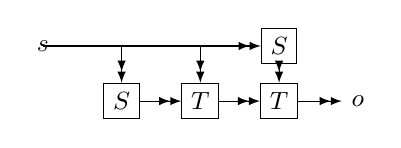
\begin{tikzpicture}[auto,>=latex]
  \node[] (input) {$s$};
  \node[] [right of=input] (dummy) {};
  \node[block, below of=dummy, node distance=.7cm] (S1) {$S$};
  \node[block, right of=S1] (T1) {$T$};
  \node[block, right of=T1] (T2) {$T$};
  \node[block, above of=T2, node distance=.7cm] (S2) {$S$};
  \node[right of=T2] (output) {$o$};
  \draw[->>] (input) -| (S1);
  \draw[->>] (input) -| (T1);
  \draw[->>] (S1) -- (T1);
  \draw[->>] (T1) -- (T2);
  \draw[->>] (input) |- (S2);
  \draw[->>] (T2) -- (output);
  \draw[->>] (S2) -- (T2);
\end{tikzpicture}
\end{center}

%\begin{definition}(lifting)
Given a function $f: A \to B$, we define a stream operator $\lift{f}
:\stream{A} \to \stream{B}$ (read as $f$ lifted) by applying function
$f$ to the input stream(s) independently at each point in time.
\begin{center}
  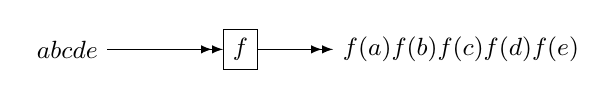
\begin{tikzpicture}[auto,>=latex]
    \node[] (input) {$\sv{a b c d e}$};
    \node[block, right of=input, node distance=2.2cm] (f) {$\lift{f}$};
    \node[right of=f, node distance=2.8cm] (output) {$\sv{f(a) f(b) f(c) f(d) f(e)}$};
    \draw[->>] (input) -- (f);
    \draw[->>] (f) -- (output);
  \end{tikzpicture}
\end{center}
%\end{definition}

We say that two \dbsp programs are \defined{equivalent} if they
compute the same input-output function on streams.  We use the symbol
$\cong$ to indicate circuit equivalence.  For example, we
can prove the following circuit equivalence (where $\circ$ is function
composition):

\noindent
\begin{tabular}{m{3.5cm}m{.3cm}m{3.5cm}}
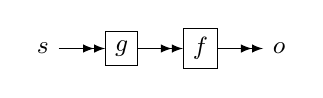
\begin{tikzpicture}[auto,>=latex]
  \node[] (input) {$s$};
  \node[block, right of=input] (g) {$\lift{g}$};
  \node[block, right of=g] (f) {$\lift{f}$};
  \node[right of=f] (output) {$o$};
  \draw[->>] (input) -- (g);
  \draw[->>] (g) -- (f);
  \draw[->>] (f) -- (output);
\end{tikzpicture}
&
$\cong$
&
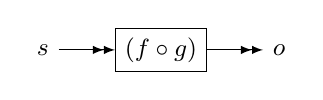
\begin{tikzpicture}[auto,>=latex]
    \node[] (input) {$s$};
    \node[block, right of=input, node distance=1.5cm] (fg) {$\lift{(f \circ g)}$};
    \node[right of=fg, node distance=1.5cm] (output) {$o$};
    \draw[->>] (input) -- (fg);
    \draw[->>] (fg) -- (output);
\end{tikzpicture}
\end{tabular}

To simplify the notation, we will write $a + b$ for streams $a, b$
instead of $a (\lift{+}) b$; we will also write $-a$ instead of
$(\lift{-})a$.

\subsection{Useful stream operators}\label{sec:abelian}

For the rest of this paper we require the set of values $A$ of a
stream $\stream{A}$ to form a commutative group, with operations $+$,
$-$, and a $0$ (zero) value.  The \emph{plus} defines what it means to
\emph{add} new data, while the \emph{minus} allows us to compute
differences (deltas).  We show later that this requirement is not a
problem for using \dbsp in the context of databases.

%\subsubsection{Delays}\label{sec:delay}

%\begin{definition}[Delay]
The \defined{delay operator} $z^{-1}$ produces an output stream by
delaying its input by one step (and starting with a
zero)\footnote{This bizarre name comes from digital signal
processing.}:

  \begin{center}
  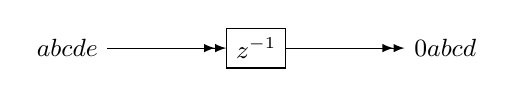
\begin{tikzpicture}[auto,>=latex,node distance=2.4cm]
    \node[] (input) {$\sv{a b c d e}$};
    \node[block, right of=input] (z) {$z^{-1}$};
    \node[right of=z] (output) {$\sv{0 a b c d}$};
    \draw[->>] (input) -- (z);
    \draw[->>] (z) -- (output);
  \end{tikzpicture}
  \end{center}
%\end{definition}

%\begin{definition}[Time invariance]
%A stream operator $S: \stream{A} \to \stream{B}$ is \defined{time-invariant} (TI) if
%$S(\zm_A(s)) = \zm_B(S(s))$ for all $s \in \stream{A}$; in other words, if
%the following two circuits are equivalent:
%
%\begin{tabular}{m{3cm}m{.5cm}m{3cm}}
%\begin{tikzpicture}[auto,>=latex]
%  \node[] (input) {$s$};
%  \node[block, right of=input] (S) {$S$};
%  \node[block, right of=S] (z) {$\zm$};
%  \node[right of=z] (output) {$o$};
%  \draw[->] (input) -- (S);
%  \draw[->] (S) -- (z);
%  \draw[->] (z) -- (output);
%\end{tikzpicture}
%&
%$\cong$
%&
%\begin{tikzpicture}[auto,>=latex]
%  \node[] (input) {$s$};
%  \node[block, right of=input] (z) {$\zm$};
%  \node[block, right of=z] (S) {$S$};
%  \node[right of=S] (output) {$o$};
%  \draw[->] (input) -- (z);
%  \draw[->] (z) -- (S);
%  \draw[->] (S) -- (output);
%\end{tikzpicture}
%\end{tabular}
%
%\noindent
%This definition extends
%naturally to operators with multiple inputs.
%\end{definition}
%
%The composition of TI operators of any number of inputs
%is TI. The delay operator $\zm$ is TI.
%\dbsp only uses TI operators.
%
%%\begin{definition}
%%We say that a function between groups $f: A \to B$ has the \emph{zero-preservation
%%property} if $f(0_A) = 0_B$.  We write $\zpp{f}$.
%%\end{definition}
%%
%%A lifted operator $\lift{f}$ is TI iff $\zpp{f}$.
%
%\subsubsection{Causal and strict operators}\label{sec:causal}
%
%\begin{definition}[Causality]
%A stream operator $S:\stream{A}\to\stream{B}$
%is \defined{causal} when for all $s,s'\in\stream{A}$,
%and all times $t$ we have:
%$
%(\forall i \leq t . s[i]=s'[i]) ~~\Rightarrow~~ S(s)[t]=S(s')[t].
%$
%\end{definition}
%
%\noindent
%In other words, the output value at time $t$ can only depend on
%input values from times $t' \leq t$.
%Operators produced by lifting are causal, and $\zm$ is causal.
%All \dbsp operators are causal.  The composition
%of causal operators of any number of inputs is causal.
%
%\begin{definition}[Strictness]
%A stream operator, $F:\stream{A}\to\stream{B}$
%is \defined{strict}
%if  $\forall s,s'\in\stream{A}, \forall t \in \N$ we have:
%$(\forall i<t . ~s[i]=s'[i]) ~~\Rightarrow \\ F(s)[t]=F(s')[t].$
%\end{definition}
%
%In other words, the $t$-th output of $F(s)$ can depend only on ``past'' values
%of the input $s$, between $0$ and $t-1$.
%In particular, $F(s)[0] = 0_B$ is the same for all $s \in \stream{A}$.
%Strict operators are causal. Lifted operators in general are \emph{not} strict.
%$\zm$ is strict.  %In \dbsp $\zm$ is the only primitive strict operator.
%
%\begin{proposition}
%\label{prop-unique-fix}
%For a strict $F: \stream{A} \to \stream{A}$ the equation ~$\alpha=F(\alpha)$~ has a unique
%solution $\alpha \in \stream{A}$, denoted by $\fix{\alpha}{F(\alpha)}$.
%\end{proposition}
%
%Thus every strict operator from a set to itself has a unique fixed
%point.  The simple proof relies on strong induction, showing that the
%solution $\alpha[t]$ depends only on the values of $\alpha$ prior to
%$t$.
%
%Consider a circuit with a strict feedback edge:
%\begin{center}
%\begin{tikzpicture}[>=latex]
%    \node[] (input) {$s$};
%    \node[block, right of=input] (f) {$T$};
%    \node[right of=f] (output) {$\alpha$};
%    \node[block, below of=f, node distance=.5cm] (z) {$F$};
%    \draw[->] (input) -- (f);
%    \draw[->] (f) -- node (mid) {} (output);
%    \draw[->] (mid.center) |-  (z);
%    \draw[->] (z.west) -- ++(-.3,0) |- ([yshift=1mm]f.south west);
%\end{tikzpicture}
%\end{center}
%
%This circuit is a well-defined function on streams:
%
%%\begin{lemma}
%%\label{lemma-causal-strict}
%%If $F: \stream{B} \to \stream{B}$ is strict and $T: \stream{A} \times \stream{B} \to \stream{B}$ is causal, then for fixed $s$ the operator
%%$\lambda\alpha.T(s,F(\alpha)): \stream{A} \to \stream{B}$ is strict.
%%\end{lemma}
%
%\begin{lemma}\label{feedback-semantics}
%\label{cor-loop}
%If $F: \stream{B} \to \stream{B}$ is strict and $T: \stream{A} \times \stream{B} \to \stream{B}$ is causal,
%the operator $Q(s)=\fix{\alpha}{T(s,F(\alpha))}$ is well-defined and causal.
%If, moreover, $F$ and $T$ are TI then so is $Q$.
%\end{lemma}
%
%All \dbsp computations are built using just lifted functions and
%delays.  We add two more operators in \secref{sec:nested}.
%
%\subsection{Integration and differentiation}\label{sec:abelianstreams}

%Remember that we require the elements of a stream to come from an abelian group $A$.
%Streams themselves form an abelian group:
%
%\begin{proposition}
%The structure $(\stream{A},+,0,-)$, obtained by lifting the $+$ and unary $-$ operations of $A$,
%is an abelian group.  0 is the stream with all values $0_A$.
%\end{proposition}
%
%\noindent
%Stream addition and negation are causal, TI operators.

%Given a linear function $f: A \to B$, the stream operator $\lift{f}$
%is linear and TI (LTI).  $\zm$ is also LTI.
%
%\begin{definition}(bilinear)
%A function of two arguments $f: A \times B \to C$ with $A, B, C$ groups, is \emph{bilinear}
%if it is linear separately in each argument (i.e., it distributes over addition):
%$\forall a, b, c, d . f(a+b, c) = f(a, c) + f(b, c)$, and $f(a, c+d) = f(a, c) + f(c, d).$
%\end{definition}
%
%This definition extends to stream operators.
%The lifting of a bilinear function $f$ is
%a bilinear stream operator $\lift{f}$.  An example
%is lifted multiplication:
%$f: \stream{\N} \times \stream{\N} \to \stream{\N}, f(a, b)[t] = a[t]\cdot b[t]$.

%The composition of (bi)linear operators with linear operators
%is (bi)linear (since homomorphisms compose).

%The ``feedback loop'' of a linear operator is linear:
%
%\begin{proposition}
%\label{prop-rec-linear}
%Let $S$ be a unary, causal, LTI operator. The
%operator $Q(s)=\fix{\alpha}{S(s+\zm(\alpha))}$ is well-defined and LTI:
%
%\begin{center}
%\begin{tikzpicture}[>=latex]
%    \node[] (input) {$s$};
%    \node[block, shape=circle, right of=input, inner sep=0pt, node distance=.6cm] (plus) {$+$};
%    \node[block, right of=plus, node distance=.6cm] (Q) {$S$};
%    \node[right of=Q, node distance=1.2cm] (output) {$\alpha$};
%    \node[block, below of=Q, node distance=.6cm] (z) {$\zm$};
%    \draw[->] (input) -- (plus);
%    \draw[->] (plus) -- (Q);
%    \draw[->] (Q) -- node (mid) {} (output);
%    \draw[->] (mid.center) |-  (z);
%    \draw[->] (z) -| (plus);
%\end{tikzpicture}
%\end{center}
%\end{proposition}

%\begin{definition}[Differentiation]
We can define \defined{differentiation operator} as a composition of
several other operators: $\D(s) \defn s - \zm(s)$, show as:

\begin{center}
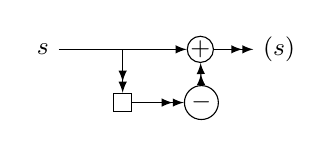
\begin{tikzpicture}[auto,>=latex,node distance=1cm]
    \node[] (input) {$s$};
    \node[block, shape=circle, right of=input, inner sep=0pt,node distance=2cm] (plus) {$+$};
    \node[right of=plus] (output) {$\D(s)$};
    \draw[draw,->] (input) -- node (i) {} (plus);
    \node[block, below of=i, node distance=.8cm] (z) {$\zm$};
    \node[block, shape=circle, right of=z, inner sep=1pt] (minus) {$-$};
    \draw[->>] (plus) -- (output);
    \draw[->>] (i) -- (z);
    \draw[->>] (z) -- (minus);
    \draw[->>] (minus) -- (plus);
\end{tikzpicture}
\end{center}
%\end{definition}
%We generally omit the type, and write just $\D$.
%The value of $\D(s)[t] = s[t] - s[t-1]$ if $t > 0$.

If $s$ is a stream, then $\D(s)$ is the \emph{stream of changes} of
$s$; a value in the output is the difference between two consecutive
values in the input.  As an example, $\D(\sv{0 1 2 3 4 5}) = \sv{0 1 1
  1 1}$.

%\begin{proposition}
%\label{prop-diff-properties}
%$\D$ is causal and LTI.
%\end{proposition}

%The integration operator ``reconstitutes'' a stream from its changes:

%\begin{definition}[Integration]
The \defined{integration operator}
is given by the following circuit:
\begin{center}
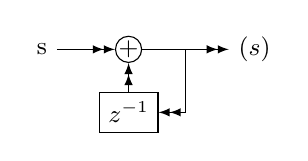
\begin{tikzpicture}[auto,>=latex, node distance=1.1cm]
    \node[] (input) {s};
    \node[block, shape=circle, right of=input, inner sep=0pt] (plus) {$+$};
    \node[right of=plus, node distance=1.6cm] (output) {$\I(s)$};
    \node[block, below of=plus, node distance=.8cm] (z) {$z^{-1}$};
    \draw[->>] (input) -- (plus);
    \draw[->>] (plus) -- node (o) {} (output);
    \draw[->>] (o) |- (z);
    \draw[->>] (z) -- (plus);
\end{tikzpicture}
\end{center}
%\end{definition}

While this definition may seem strange, because the output stream is
used to compute itself, the use of the delay in the ``feedback'' loop
ensures that only ``previous'' values of the output are used in
computing the current one, so this circuit is really well-defined.
%\noindent
%We also generally omit the type, and write just $\I$.
%This is the construction from Proposition~\ref{prop-rec-linear}
%using the identity function for $S$.
%
%\begin{proposition}
%$\I(s)$ is the discrete (indefinite) integral applied to the stream $s$:
%\end{proposition}
In general, $\I(s)[t] = \sum_{i \leq t} s[i]$.
As an example, $\I(\sv{0 1 2 3 4 5}) = \sv{0 1 3 6 10}$.

%\begin{proposition}
%\label{prop-integ-properties}
%$\I$ is causal and LTI.
%\end{proposition}
%
%\begin{theorem}[Inversion]
%\label{inverses}
%Integration and differentiation are inverses of each other:
%$\forall s . \I(\D(s)) = \D(\I(s)) = s$.
%\end{theorem}

Integration and differentiation ``cancel'' each other:

\noindent
\begin{tabular}{m{2.5cm}m{.3cm}m{1cm}m{.3cm}m{2.5cm}}
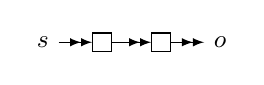
\begin{tikzpicture}[auto,>=latex, node distance=.75cm]
    \node[] (input) {$s$};
    \node[block, right of=input] (I) {$\I$};
    \node[block, right of=I] (D) {$\D$};
    \node[right of=D] (output) {$o$};
    \draw[->>] (input) -- (I);
    \draw[->>] (I) -- (D);
    \draw[->>] (D) -- (output);
\end{tikzpicture}
     &
     $\cong$
     &
     \hspace{-2ex}
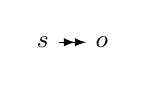
\begin{tikzpicture}[auto,>=latex, node distance=.75cm]
    \node[] (input) {$s$};
    \node[right of=input] (output) {$o$};
    \draw[->>] (input) -- (output);
\end{tikzpicture}
     &
     $\cong$
     &
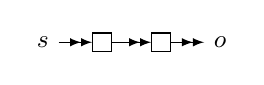
\begin{tikzpicture}[auto,>=latex, node distance=.75cm]
    \node[] (input) {$s$};
    \node[block, right of=input] (D) {$\D$};
    \node[block, right of=D] (I) {$\I$};
    \node[right of=I] (output) {$o$};
    \draw[->>] (input) -- (D);
    \draw[->>] (D) -- (I);
    \draw[->>] (I) -- (output);
\end{tikzpicture}
\end{tabular}

\section{Incremental view maintenance}\label{sec:incremental}

%Here we define IVM and analyze its properties.

%\begin{definition}
Given a stream operator $Q: \stream{A} \to \stream{B}$ we define the
\defined{incremental version} of $Q$ as:
%\begin{equation}\label{def:inc}
%\inc{Q} \defn \D \circ Q \circ \I.
%\end{equation}
%$\inc{Q}$ has the same ``type'' as $Q$: $\inc{Q}: \stream{A} \to \stream{B}$.
%For an operator with multiple inputs we define
%the incremental version by applying $\I$ to each input independently:
%e.g., if $T: \stream{A} \times \stream{B} \rightarrow \stream{C}$ then
%$\inc{T}(a, b) \defn \D (T(\I(a), \I(b)))$.

%The following diagram illustrates the intuition behind this
%definition:
\vspace{-2ex}
\begin{center}
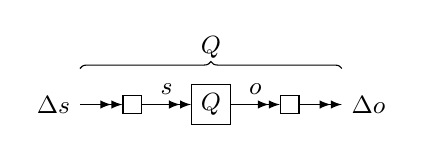
\begin{tikzpicture}[auto,>=latex]
    \node[] (input) {$\Delta s$};
    \node[block, right of=input] (I) {$\I$};
    \node[block, right of=I] (Q) {$Q$};
    \node[block, right of=Q] (D) {$\D$};
    \node[right of=D] (output) {$\Delta o$};
    \draw[->>] (input) -- (I);
    \draw[->>] (I) -- node (s) {$s$} (Q);
    \draw[->>] (Q) -- node (o) {$o$} (D);
    \draw[->>] (D) -- (output);
    \draw[decorate, decoration = {brace, raise=13pt}] (input) -- (output)
    node[pos=.5, above=13pt]{$\inc{Q}$};
\end{tikzpicture}
\end{center}
%\end{definition}

If $Q$ computes on a stream $s$, then $\inc{Q}$ computes on a stream
of changes to $s$.  If $Q$ produces a stream $o$, then $\inc{Q}$
produces the stream of changes to $o$.
%Notice that our definition of incremental computation is meaningful only for \emph{streaming}
%computations; this is in contrast to classic definitions, e.g.~\cite{gupta-idb95} which
%consider only one change.  Generalizing the definition to operate on streams gives us
%additional power, especially when operating with recursive queries.
%
%The following proposition is one of our central results:
$\inc{Q}$ has many nice properties:

%\begin{proposition}(Properties of the incremental version):
%\label{prop-inc-properties}
%\begin{description}
%\item[inversion:] $Q\mapsto\inc{Q}$ is bijective; its inverse is $Q\mapsto \I\circ Q\circ\D$.
%\item[invariance:] $\inc{+} = +, \inc{(\zm)} = \zm, \inc{-} = -, \inc{\I}=\I, \inc{\D}=\D$
%\item[push/pull:] \label{prop-part-commutation}
%    $Q \circ \I = \I \circ \inc{Q}$; $\D\circ Q = \inc{Q}\circ\D$
%\item[chain:] $\inc{(Q_1\circ Q_2)} = \inc{Q_1}\circ\inc{Q_2}$ (Generalizes to multiple inputs.)
%\item[add:] $\inc{(Q_1 + Q_2)} = \inc{Q_1} + \inc{Q_2}$
%\item[cycle:] $\inc{(\lambda s. \fix{\alpha}{T(s,\zm(\alpha)}))} = \lambda s. \fix{\alpha}{\inc{T}(s,\zm(\alpha)})$
%\end{description}
%\end{proposition}
%
The \defined{chain rule} states that $\inc{(Q_1 \circ Q_2)} =
\inc{Q_1} \circ \inc{Q_2}$, i.e., these circuits are equivalent:

\noindent
\begin{tabular}{rr}
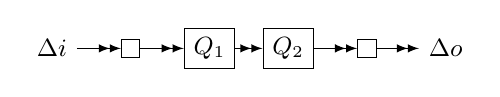
\begin{tikzpicture}[auto,>=latex]
  \node[] (input) {$\Delta i$};
  \node[block, right of=input] (I) {$\I$};
  \node[block, right of=I] (Q1) {$Q_1$};
  \node[block, right of=Q1] (Q2) {$Q_2$};
  \node[block, right of=Q2] (D) {$\D$};
  \node[right of=D] (output)  {$\Delta o$};
  \draw[->>] (input) -- (I);
  \draw[->>] (I) -- (Q1);
  \draw[->>] (Q1) -- (Q2);
  \draw[->>] (Q2) -- (D);
  \draw[->>] (D) -- (output);
\end{tikzpicture} &
$\cong$ \\
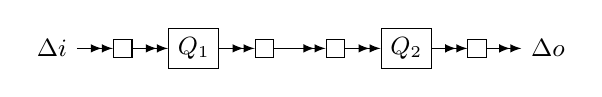
\begin{tikzpicture}[>=latex, node distance=.9cm]
  \node[] (input) {$\Delta i$};
  \node[block, right of=input] (I1) {$\I$};
  \node[block, right of=I1] (Q1) {$Q_1$};
  \node[block, right of=Q1] (D1) {$\D$};
  \node[block, right of=D1] (I2) {$\I$};
  \node[block, right of=I2] (Q2) {$Q_2$};
  \node[block, right of=Q2] (D2) {$\D$};
  \node[right of=D2] (output)  {$\Delta o$};
  \draw[->>] (input) -- (I1);
  \draw[->>] (I1) -- (Q1);
  \draw[->>] (Q1) -- (D1);
  \draw[->>] (D1) -- (I2);
  \draw[->>] (I2) -- (Q2);
  \draw[->>] (Q2) -- (D2);
  \draw[->>] (D2) -- (output);
\end{tikzpicture} &
$\cong$ \\
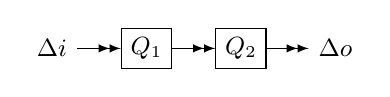
\begin{tikzpicture}[>=latex, node distance=1.2cm]
  \node[] (input) {$\Delta i$};
  \node[block, right of=input] (Q1) {$\inc{Q_1}$};
  \node[block, right of=Q1] (Q2) {$\inc{Q_2}$};
  \node[right of=Q2] (output)  {$\Delta o$};
  \draw[->>] (input) -- (Q1);
  \draw[->>] (Q1) -- (Q2);
  \draw[->>] (Q2) -- (output);
\end{tikzpicture}
\end{tabular}

\noindent In other words, \textbf{to incrementalize a composite query
  you can incrementalize each sub-query independently}.  This gives us
a simple deterministic recipe for computing the incremental version of
an arbitrarily complex query.

The \defined{cycle rule} states that these circuits are equivalent:

\noindent
\begin{tabular}{m{4.4cm}m{.2cm}m{3cm}}
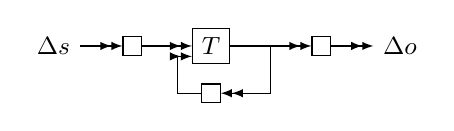
\begin{tikzpicture}[>=latex]
    \node[] (input) {$\Delta s$};
    \node[block, right of=input] (I) {$\I$};
    \node[block, right of=I] (f) {$T$};
    \node[block, right of=f, node distance=1.4cm] (D) {$\D$};
    \node[right of=D] (output) {$\Delta o$};
    \node[block, below of=f, node distance=.6cm] (z) {$\zm$};
    \draw[->>] (input) -- (I);
    \draw[->>] (I) -- (f);
    \draw[->>] (f) -- node (mid) {} (D);
    \draw[->>] (mid.center) |-  (z);
    \draw[->>] (z.west) -- ++(-.3,0) |- ([yshift=1mm]f.south west);
    \draw[->>] (D) -- (output);
\end{tikzpicture} & $\cong$ &
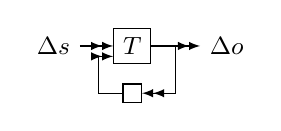
\begin{tikzpicture}[>=latex]
    \node[] (input) {$\Delta s$};
    \node[block, right of=input] (f) {$\inc{T}$};
    \node[right of=f, node distance=1.2cm] (output) {$\Delta o$};
    \node[block, below of=f, node distance=.6cm] (z) {$\zm$};
    \draw[->>] (input) -- (f);
    \draw[->>] (f) -- node (mid) {} (output);
    \draw[->>] (mid.center) |-  (z);
    \draw[->>] (z.west) -- ++(-.3,0) |- ([yshift=1mm]f.south west);
\end{tikzpicture}
\end{tabular}

In other words, the incremental version of a feedback loop around a query
is just the feedback loop with the incremental query for its body.
This result will be useful when we implement recursive queries.

%To execute incremental queries efficiently, we want to compute directly
%on streams of changes, without integrating them. The invariance property above shows
%that stream operators $+$, $-$, and $\zm$ are identical to their incremental versions.
%The following theorems generalize this to linear and bi-linear operators:

We call an operator $Q$ \defined{linear} if it has the property that
$Q(a+b) = Q(a) + Q(b)$ (where $+$ is the addition of streams).

%\begin{theorem}[Linear]\label{linear}
For a linear operator $Q$ we have $\inc{Q}=Q$.
%\end{theorem}

This is a very useful fact, because many database operations can be
implemented as linear operators.  We will see that in databases
selection, projection, filtering, grouping, parts of aggregation are
all linear.  Moreover, many of the operators we have seen so far are
linear: $-$, $z^{-1}$, $\I$, $\D$, $\lift{f}$ if $f$ is a linear
function.

We call an operator with two inputs $Q$ \defined{bilinear} if it
distributes over stream addition: $Q(a+b, c) = Q(a, c) + Q(b, c)$, and
$Q(a, c+d) = Q(a, c) + Q(a, d)$.  (This is similar how multiplication
distributes over addition.)  In databases intersection, joins, and
Cartesian products are bilinear.

%\begin{theorem}[Bilinear]\label{bilinear}
For a bilinear operator $\times$ we have:
\begin{eqnarray*}
\inc{(\Delta a \times \Delta b)} = \\
(\Delta a \times \Delta b ~+~ \zm(\I(\Delta a)) \times
\Delta b ~+~ \Delta a \times \zm(\I(\Delta b)) = \\
\Delta a \times \Delta b + \zm(a) \times \Delta b + \Delta a \times \zm(b)
\end{eqnarray*}

%In pictures: \\
\noindent
\begin{tabular}{m{3.3cm}m{0cm}m{4cm}%m{0cm}m{2.8cm}
  }
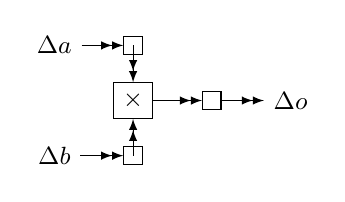
\begin{tikzpicture}[auto,>=latex]
    \node[] (a) {$\Delta a$};
    \node[block, right of=a] (ai) {$\I$};
    \node[below of=a, node distance=.7cm] (midway) {};
    \node[below of=midway, node distance=.7cm] (b) {$\Delta b$};
    \node[block, right of=b] (bi) {$\I$};
    \node[block, right of=midway, node distance=1cm] (q) {$\times$};
    \node[block, right of=q] (D) {$\D$};
    \node[right of=D] (output) {$\Delta o$};
    \draw[->>] (a) -- (ai);
    \draw[->>] (b) -- (bi);
    \draw[->>] (ai) -| (q);
    \draw[->>] (bi) -| (q);
    \draw[->>] (q) -- (D);
    \draw[->>] (D) -- (output);
\end{tikzpicture} &
$\cong$ &
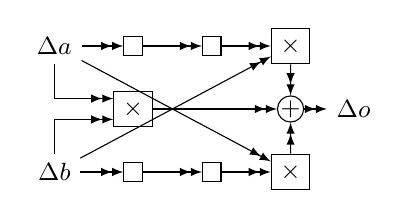
\begin{tikzpicture}[auto,>=latex]
  \node[] (input1) {$\Delta a$};
  \node[below of=input1, node distance=1.6cm] (input2) {$\Delta b$};
  \node[block, right of=input1, node distance=1cm] (I1) {$\I$};
  \node[block, below of=I1,node distance=.8cm] (ab) {$\times$};
  \node[block, right of=input2, node distance=1cm] (I2) {$\I$};
  \draw[->>] (input1) -- (I1);
  \draw[->>] (input2) -- (I2);
  \draw[->>] (input1) |- ([yshift=-1mm]ab.north west);
  \draw[->>] (input2) |- ([yshift=1mm]ab.south west);
  \node[block, right of=I1] (ZI1) {$\zm$};
  \node[block, right of=I2] (ZI2) {$\zm$};
  \draw[->>] (I1) -- (ZI1);
  \draw[->>] (I2) -- (ZI2);
  \node[block, right of=ZI1] (DI1) {$\times$};
  \node[block, right of=ZI2] (DI2) {$\times$};
  \draw[->>] (ZI1) -- (DI1);
  \draw[->>] (ZI2) -- (DI2);
  \node[block, circle, right of=ab, inner sep=0cm, node distance=2cm] (sum) {$+$};
  \draw[->>] (ab) -- (sum);
  \draw[->>] (DI1) -- (sum);
  \draw[->>] (DI2) -- (sum);
  \node[right of=sum, node distance=.8cm] (output) {$\Delta o$};
  \draw[->>] (sum) -- (output);
  \draw[->>] (input1) -- (DI2);
  \draw[->>] (input2) -- (DI1);
\end{tikzpicture}
%&
%$\cong$ &
%\begin{tikzpicture}[auto,>=latex,node distance=.7cm]
%  \node[] (input1) {$a$};
%  \node[below of=input1, node distance=1cm] (input2) {$b$};
%  \node[block, right of=input1, node distance=.5cm] (I1) {$\I$};
%  \node[block, right of=input2, node distance=.5cm] (I2) {$\I$};
%  \draw[->>] (input1) -- (I1);
%  \draw[->>] (input2) -- (I2);
%  \node[block, right of=I2] (ZI2) {$\zm$};
%  \draw[->>] (I2) -- (ZI2);
%  \node[block, right of=I1] (DI1) {$\times$};
%  \node[block, right of=ZI2] (DI2) {$\times$};
%  \draw[->>] (I1) -- (DI1);
%  \draw[->>] (ZI2) -- (DI2);
%  \node[block, circle, above of=DI2, inner sep=0cm, node distance=.5cm] (sum) {$+$};
%  \draw[->>] (DI1) -- (sum);
%  \draw[->>] (DI2) -- (sum);
%  \node[right of=sum, node distance=.5cm] (output) {$o$};
%  \draw[->>] (sum) -- (output);
%  \draw[->>] (input1) -- (DI2);
%  \draw[->>] (input2) -- (DI1);
%\end{tikzpicture}
\end{tabular}
%\end{theorem}

What is the intuition behind this diagram?  Let us consider the case
of Cartesian product $a \times b$.  The incremental product has inputs
$\Delta a = \D(a)$ and $\Delta b = \D(b)$.

What happens when we add a row $x$ to relation $a$ (i.e., $\Delta a =
x$)?  How does the output change?  The new row $x$ will appear
combined with every row in the \emph{previous version} of the
\emph{full} relation $b$.  The operator $\I(\Delta b)$ in fact
computes relation $b$ from the stream $\Delta b$ of changes, and $\zm$
applied to this value gives us its previous version.  So the bottom
$\times$ operator computes $x \times \zm(b) = \Delta a \times
\zm(\I(\Delta b))$, the change produced by the new row $x$.  The top
$\times$ operator performs the symmetric operation for the changes of
the $b$ relation.  And the middle $\times$ operator produces results
when changes happen to both relations.

%Rewriting this statement using $\Delta a$ for the stream of changes to
%$a$ we get the familiar formula for incremental equi-joins:
%$\Delta(a\times b) =\Delta a \times \Delta b + a\times(\Delta b) +
%(\Delta a)\times b$; equi-joins are indeed bilinear.
%

\input{relational}
\section{Recursive queries}\label{sec:recursion}

Recursive queries are very useful in a many applications.
For example, graph algorithms such as graph reachability
or transitive closure are naturally expressed using recursive queries.

We introduce two simple \dbsp stream operators that are used for
expressing recursive query evaluation.  These operators allow us
to build circuits implementing looping constructs, which
are used to iterate computations until a fixed-point is reached.
The following definition allows us to describe what a fixed point is
in terms of streams:

\begin{definition}\label{def:zae}
We say that a stream $s \in \stream{A}$ is \defined{zero almost-everywhere} if it has a finite
number of non-zero values, i.e., there exists a time $t_0 \in \N$
s.t. $\forall t \geq t_0 . s[t] = 0$.
\noindent Denote the set of streams that are zero almost everywhere
by $\streamf{A} \subset \stream{A}$.
\end{definition}

\paragraph{Stream introduction}

The delta function (named from the Dirac delta function) $\delta : A \rightarrow \stream{A}$
produces a stream from a scalar value:
$$\delta(v)[t] \defn \left\{
\begin{array}{ll}
  v & \mbox{if } t = 0 \\
  0_A & \mbox{ otherwise}
\end{array}
\right.
$$

The input of $\delta$ has a single arrow, while the output has a
double arrow.  For example:

\begin{center}
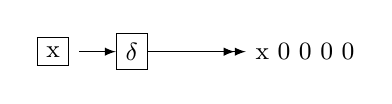
\begin{tikzpicture}[auto,node distance=1cm,>=latex]
    \node[] (input) {\fbox{x}};
    \node[block, right of=input] (delta) {$\delta$};
    \node[right of=delta, node distance=2.2cm] (output) {\sv{x 0 0 0 0}};
    \draw[->] (input) -- (delta);
    \draw[->>] (delta) -- (output);
\end{tikzpicture}
\end{center}

\paragraph{Stream elimination}

We define the function $\int : \streamf{A} \rightarrow A$, over
streams that are zero almost everywhere, as $\int(s) \defn \sum_{t
  \geq 0} s[t]$.  $\int$ simply adds up all values in the input stream
and produces a scalar result with the sum.  $\int$ is closely related
to $\I$; if $\I$ is the indefinite (discrete) integral, $\int$ is the
definite (discrete) integral on the interval $0 - \infty$.  For
example, $\int(\sv{1 2 3 0 0}) = 6$.

In circuits constructed for many classes of queries, including
relational and Datalog queries given below, the $\int$ operator can be
``approximated'' without loss of precision by integrating until it
encounters the first 0.

Notice that the input of $\int$ is a double arrow, while the output is
a single arrow.  E.g.,:

\begin{center}
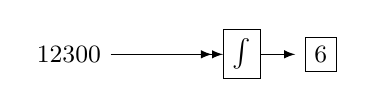
\begin{tikzpicture}[auto,node distance=1cm,>=latex]
    \node[] (input) {$\sv{1 2 3 0 0}$};
    \node[block, right of=input, node distance=2.2cm] (S) {$\int$};
    \node[right of=S] (output) {$\fbox{6}$};
    \draw[->>] (input) -- (S);
    \draw[->] (S) -- (output);
\end{tikzpicture}
\end{center}

%$\delta$ is the left inverse of $\int$, i.e.: $\int \circ \; \delta = \id_A$.
\begin{proposition}
$\delta$ and $\int$ are LTI.
\end{proposition}

\paragraph{Nested time domains}

So far we have used a tacit assumption that ``time'' is common for all
streams in a program.  For example, when we add two streams,
we assume that they use the same ``clock'' for the time dimension.
However, the $\delta$ operator creates a stream with a ``new'', independent time
dimension.  We require \emph{well-formed circuits}
to ``insulate'' such
nested time domains by ``bracketing'' them between a $\delta$
and an $\int$ operator:

\begin{center}
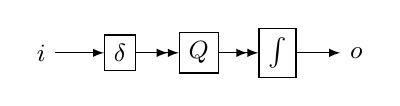
\begin{tikzpicture}[auto,node distance=1cm,>=latex]
    \node[] (input) {$i$};
    \node[block, right of=input] (delta) {$\delta$};
    \node[block, right of=delta] (f) {$Q$};
    \draw[->] (input) -- (delta);
    \draw[->>] (delta) -- (f);

    \node[block, right of=f] (S) {$\int$};
    \node[right of=S] (output) {$o$};
    \draw[->>] (f) -- (S);
    \draw[->] (S) -- (output);
\end{tikzpicture}
\end{center}

In the above circuit $Q$ is a streaming operator, but the entire
circuit is a scalar function, shown by the single input and output
arrows.

Algorithm~\ref{algorithm-rec} below, which translates recursive queries to
\dbsp circuits, always produces well-formed circuits.
%\begin{proposition}
%If $Q$ is time-invariant, the circuit above has the zero-preservation
%property: $\zpp{\int \circ\; Q \circ \delta_o}$.
%\end{proposition}

\subsection{Implementing recursive queries}\label{sec:datalog}

We describe the implementation of recursive queries in \dbsp for
stratified Datalog.
In general, a recursive Datalog program defines a set of
mutually recursive relations $O_1,..,O_n$ as an equation
$(O_1,..,O_n)=R(I_1,..,I_m, O_1,..,O_n)$, where $I_1,..,I_m$ are
input relations and $R$ is a non-recursive query.

We describe here the algorithm for the simpler case of a single-input,
single-output query\footnote{The general case in the companion
technical report~\cite{tr} is only slightly more involved.}.  The
input of our algorithm is a Datalog query of the form $O = R(I, O)$,
where $R$ is a relational, non-recursive query, producing a set as a
result, but whose output $O$ is also an input.  The output of the
algorithm is a \dbsp circuit which evaluates this recursive query
producing output $O$ when given the input $I$.  In this section we
build a non-incremental circuit, which evaluates the Datalog query; in
\refsec{sec:nested} we incrementalize this circuit.

\begin{algorithm}%[recursive queries]
  \label{algorithm-rec}
\noindent
\begin{enumerate}[nosep, leftmargin=\parindent]
\item Implement the non-recursive relational query $R$ as described in
    \secref{sec:relational} and Table~\ref{tab:relational}; this produces
    an acyclic circuit whose inputs and outputs are \zrs:
    \begin{center}
    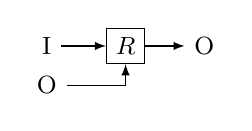
\begin{tikzpicture}[auto,>=latex]
      \node[] (I) {\code{I}};
      \node[below of=I, node distance=.5cm] (O) {\code{O}};
      \node[block, right of=I] (R) {$R$};
      \node[right of=R] (o) {\code{O}};
      \draw[->] (I) -- (R);
      \draw[->] (O) -| (R);
      \draw[->] (R) -- (o);
    \end{tikzpicture}
    \end{center}

In all these diagrams we show input 0 of operator $R$ on the left, and
input 1 on the bottom.

\item Lift this circuit to operate on streams:
    \begin{center}
    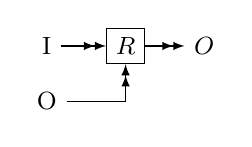
\begin{tikzpicture}[auto,>=latex]
      \node[] (I) {\code{I}};
      \node[below of=I, node distance=.7cm] (O) {\code{O}};
      \node[block, right of=I] (R) {$\lift R$};
      \node[right of=R] (o) {$O$};
      \draw[->>] (I) -- (R);
      \draw[->>] (O) -| (R);
      \draw[->>] (R) -- (o);
    \end{tikzpicture}
    \end{center}

  We construct $\lift{R}$ by lifting each operator of the circuit individually
  according to Proposition~\ref{prop:distributivity}.

\item Build a cycle, connecting the output to the corresponding
recursive input via a delay:

 \begin{center}
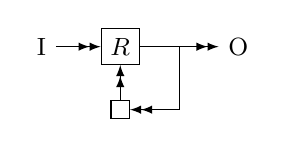
\begin{tikzpicture}[auto,>=latex, node distance=.8cm]
  \node[] (I) {\code{I}};
  \node[block, right of=I, node distance=1cm] (R) {$\lift R$};
  \node[right of=R, node distance=1.5cm] (O) {\code{O}};
  \node[block, below of=R, node distance=.8cm] (z) {$\zm$};
  \draw[->>] (I) -- (R);
  \draw[->>] (R) -- node(o) {} (O);
  \draw[->>] (o) |- (z);
  \draw[->>] (z) -- (R);
 \end{tikzpicture}
 \end{center}

\item ``Bracket'' the circuit, first with $\I$ and $\D$ nodes, and
  then in $\delta$ and $\int$:

\begin{center}
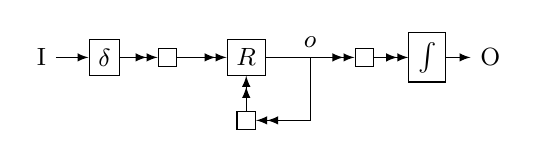
\begin{tikzpicture}[auto,>=latex, node distance=.8cm]
  \node[] (Iinput) {\code{I}};
  \node[block, right of=Iinput] (ID) {$\delta$};
  \node[block, right of=ID] (II) {$\I$};
  \node[block, right of=II, node distance=1cm] (f) {$\lift{R}$};
  \node[block, right of=f, node distance=1.5cm] (D) {$\D$};
  \node[block, right of=D] (S) {$\int$};
  \node[right of=S] (output)  {\code{O}};
  \draw[->] (Iinput) -- (ID);
  \draw[->>] (ID) -- (II);
  \draw[->>] (II) -- (f);
  \draw[->>] (f) -- node (o) {$o$} (D);
  \draw[->>] (D) -- (S);
  \draw[->] (S) -- (output);
  \node[block, below of=f, node distance=.8cm] (z) {$\zm$};
  \draw[->>] (o) |- (z);
  \draw[->>] (z) -- (f);
\end{tikzpicture}
    \vspace{-2ex}
\end{center}
\end{enumerate}
\end{algorithm}

We argue that the cycle inside this circuit computes iteratively the fixed point of $R$.
The $\D$ operator yields the set of new Datalog facts (changes) computed by each iteration of the loop.
When the set of new facts becomes empty, the fixed point has been reached:

\begin{theorem}[Recursion correctness]\label{theorem:recursion}
If $\isset(\code{I})$, the output of the circuit above is
the relation $\code{O}$ as defined by the Datalog semantics of given program
$R$ as a function of the input relation \code{I}.
\end{theorem}
\label{proof-recursion}

\begin{proof}
Let us compute the contents of the $o$ stream, produced at the output
of $R$.  We show that this stream contains increasing approximations of the value of \code{O}.

Define the following one-argument function: $S(x) = \lambda x . R(\code{I}, x)$.
Notice that the left input of the $\lift{R}$ block is a constant stream
with the value \code{I}.  Due to the stratified nature of the language,
we must have $\ispositive(S)$, so $\forall x . S(x) \geq x$.
We get the following system of equations:
$$
\begin{aligned}
o[0] =& S(0) \\
o[t] =& S(o[t-1]) \\
\end{aligned}
$$
So, by induction on $t$ we have $o[t] = S^t(0)$, where by
$S^t$ we mean $\underbrace{S \circ S \circ \ldots \circ S}_{t}$.
$S$ is monotone; thus, if there is a time $k$ such that $S^k(0) = S^{k+1}(0)$, we have
$\forall j . S^{k+j}(0) = S^k(0)$.  Applying a $\D$ to this stream
will then produce a stream that is zero almost everywhere, and integrating
this result will return the last distinct value in the stream $o$.

This is essentially the definition of the semantics of a recursive Datalog relation:
$\code{O} = \fix{x}{R(\code{I}, x)}$.\qed
\end{proof}

Note that if the query $R$ computes over unbounded data domains (e.g.,
using integers with arithmetic), this construction does not guarantee
that at runtime a fixed point is reached.  But if a program does converge, the
above construction will find the least fixed point.

In fact, this circuit implements the standard \defined{na\"{\i}ve evaluation}
algorithm (e.g., see Algorithm~1 in \cite{greco-sldm15}).
Notice that the inner part of the circuit is the incremental
form of another circuit, since it is sandwiched between $\I$ and $\D$ operators.
Using the cycle rule of Proposition~\ref{prop-inc-properties} we can rewrite this circuit as:
%
\begin{center}
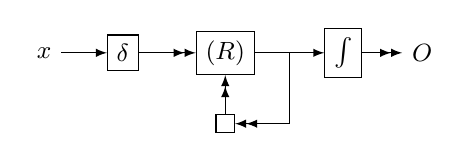
\begin{tikzpicture}[auto,>=latex]
  \node[] (Iinput) {$x$};
  \node[block, right of=Iinput] (Idelta) {$\delta$};
  \node[block, right of=Idelta, node distance=1.3cm] (f) {$\inc{(\lift{R})}$};
  \node[block, right of=f, node distance=1.5cm] (S) {$\int$};
  \node[right of=S] (output)  {$O$};
  \node[block, below of=f, node distance=.9cm] (z) {$\zm$};
  \draw[->] (Iinput) -- (Idelta);
  \draw[->] (f) -- node (o) {} (S);
  \draw[->>] (S) -- (output);
  \draw[->>] (o) |- (z);
  \draw[->>] (z) -- (f);
  \draw[->>] (Idelta) -- (f);
\end{tikzpicture}
\end{center}

This circuit implements \defined{semi-na\"{\i}ve evaluation}
(Algorithm~2 from~\cite{greco-sldm15}).  We have just proven the
correctness of semi-na\"{\i}ve evaluation as an immediate consequence
of the cycle rule!

%In \refsec{sec:recursive-example} we show a concrete example, applying Algorithm~\ref{algorithm-rec}
%to a recursive query computing the transitive closure of a graph.

\subsection{Example recursive query}\label{sec:recursive-example}

Let us apply Algorithm~\ref{algorithm-rec} to a concrete Datalog
program, which computes the transitive closure of a directed graph:

\begin{lstlisting}[language=ddlog,basicstyle=\small\ttfamily]
// Edge relation with head and tail
input relation E(h: Node, t: Node)
// Reach relation with source s and sink t
output relation R(s: Node, t: Node)
R(x, y) :- E(x, y).
R(x, y) :- E(x, z), R(z, y).
\end{lstlisting}

Step 1: we ignore the fact that R is both an input and an output and we implement
the \dbsp circuit corresponding to the body of the query.  This query could be expressed
in SQL as:

\begin{lstlisting}[language=SQL,basicstyle=\small\ttfamily]
( SELECT * FROM E )
UNION
( SELECT E.h , R.t
  FROM E JOIN R ON E.t = R.s )
\end{lstlisting}

\noindent Step 1:
This generates a circuit with inputs \code{E} and \code{R}:

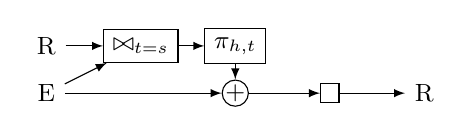
\begin{tikzpicture}[>=latex, node distance=1.2cm]
  \node[] (E) {\code{E}};
  \node[above of=E, node distance=.6cm] (R1) {\code{R}};
  \node[block, right of=R1] (j) {$\bowtie_{t=s}$};
  \node[block, right of=j] (pj) {$\pi_{h, t}$};
  \node[block, circle, below of=pj, inner sep=0cm, node distance=.6cm] (plus) {$+$};
  \node[block, right of=plus] (d) {$\distinct$};
  \node[right of=d] (R) {\code{R}};
  \draw[->] (R1) -- (j);
  \draw[->] (E) -- (j);
  \draw[->] (j) -- (pj);
  \draw[->] (E) -- (plus);
  \draw[->] (pj) -- (plus);
  \draw[->] (plus) -- (d);
  \draw[->] (d) -- (R);
\end{tikzpicture}

\noindent Step 2: Lift the circuit by lifting each operator:

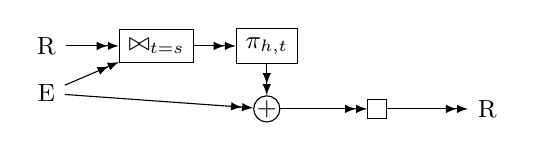
\begin{tikzpicture}[>=latex, node distance=1.4cm]
  \node[] (E) {\code{E}};
  \node[above of=E, node distance=.6cm] (R1) {\code{R}};
  \node[block, right of=R1] (j) {$\lift{\bowtie_{t=s}}$};
  \node[block, right of=j] (pj) {$\lift{\pi_{h, t}}$};
  \node[block, circle, below of=pj, node distance=.8cm, inner sep=0cm] (plus) {$+$};
  \node[block, right of=plus] (d) {$\lift{\distinct}$};
  \node[right of=d] (R) {\code{R}};
  \draw[->>] (R1) -- (j);
  \draw[->>] (E) -- (j);
  \draw[->>] (j) -- (pj);
  \draw[->>] (E) -- (plus);
  \draw[->>] (pj) -- (plus);
  \draw[->>] (plus) -- (d);
  \draw[->>] (d) -- (R);
\end{tikzpicture}

\noindent Step 3: Connect the feedback loop implied by \code{R}:

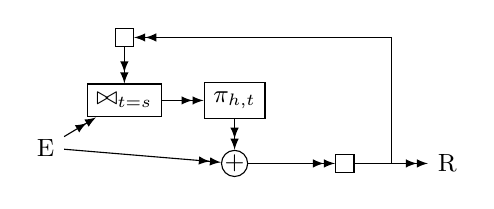
\begin{tikzpicture}[>=latex]
  \node[] (E) {\code{E}};
  \node[right of=E] (empty) {};
  \node[block, above of=empty, node distance=.6cm] (j) {$\lift{\bowtie_{t=s}}$};
  \node[block, right of=j, node distance=1.4cm] (pj) {$\lift{\pi_{h, t}}$};
  \node[block, circle, below of=pj, node distance=.8cm, inner sep=0cm] (plus) {$+$};
  \node[block, right of=plus, node distance=1.4cm] (d) {$\lift{\distinct}$};
  \draw[->>] (E) -- (j);
  \draw[->>] (j) -- (pj);
  \draw[->>] (E) -- (plus);
  \draw[->>] (pj) -- (plus);
  \draw[->>] (plus) -- (d);

  % generic part
  \node[right of=d, node distance=1.3cm] (output)  {\code{R}};
  \draw[->>] (d) -- node (o) {} (output);
  \node[block, above of=j, node distance=.8cm] (z) {$\zm$};
  \draw[->>] (o.center) |- (z);
  \draw[->>] (z) -- (j);
\end{tikzpicture}

\noindent Step 4: ``bracket'' the circuit with $\I$-$\D$, and with $\delta$-$\int$:

\noindent
\begin{tikzpicture}[>=latex, node distance=1.3cm]
  \node[] (Einput) {\code{E}};
  % generic part
  \node[block, right of=Einput, node distance=.8cm] (ID) {$\delta$};
  \node[block, right of=ID, node distance=.8cm] (E) {$\I$};

  % relational query
  \node[block, above of=E, node distance=.8cm] (j) {$\lift{\bowtie_{t=s}}$};
  \node[block, right of=j, node distance=1.4cm] (pj) {$\lift{\pi_{h, t}}$};
  \node[block, circle, below of=pj, node distance=.8cm, inner sep=0cm] (plus) {$+$};
  \node[block, right of=plus] (d) {$\lift{\distinct}$};
  \draw[->>] (E) -- (j);
  \draw[->>] (j) -- (pj);
  \draw[->>] (E) -- (plus);
  \draw[->>] (pj) -- (plus);
  \draw[->>] (plus) -- (d);

  % generic part
  \node[block, right of=d, node distance=1.3cm] (D) {$\D$};
  \node[block, right of=D, node distance=1cm] (S) {$\int$};
  \node[right of=S, node distance=.8cm] (output)  {\code{R}};
  \draw[->] (Einput) -- (ID);
  \draw[->>] (ID) -- (E);
  \draw[->>] (d) -- node (o) {} (D);
  \draw[->>] (D) -- (S);
  \draw[->] (S) -- (output);
  \node[block, above of=j, node distance=.8cm] (z) {$\zm$};
  \draw[->>] (o.center) |- (z);
  \draw[->>] (z) -- (j);
\end{tikzpicture}

The above circuit is a complete implementation of the non-streaming
recursive query; given an input relation \code{E} it will produce
its transitive closure \code{R} as output.

Now we use cycle rule to convert this circuit to seminaive evaluation
(to save space we omit indices):

\noindent
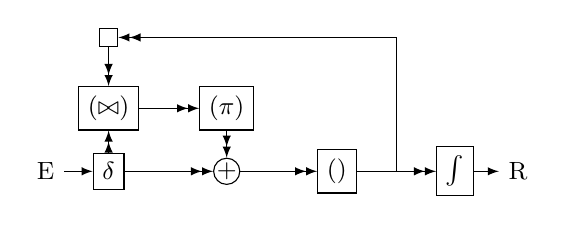
\begin{tikzpicture}[>=latex, node distance=1.4cm]
  \node[] (Einput) {\code{E}};
  % generic part
  \node[block, right of=Einput, node distance=.8cm] (E) {$\delta$};

  % relational query
  \node[block, above of=E, node distance=.8cm] (j) {$\inc{(\lift{\bowtie})}$};
  \node[block, right of=j, node distance=1.5cm] (pj) {$\inc{(\lift{\pi})}$};
  \node[block, circle, below of=pj, node distance=.8cm, inner sep=0cm] (plus) {$+$};
  \node[block, right of=plus] (d) {$\inc{(\lift{\distinct})}$};
  \draw[->>] (E) -- (j);
  \draw[->>] (j) -- (pj);
  \draw[->>] (E) -- (plus);
  \draw[->>] (pj) -- (plus);
  \draw[->>] (plus) -- (d);

  % generic part
  \node[block, right of=d, node distance=1.5cm] (S) {$\int$};
  \node[right of=S, node distance=.8cm] (output)  {\code{R}};
  \draw[->] (Einput) -- (E);
  \draw[->>] (d) -- node (o) {} (S);
  \draw[->] (S) -- (output);
  \node[block, above of=j, node distance=.9cm] (z) {$\zm$};
  \draw[->>] (o.center) |- (z);
  \draw[->>] (z) -- (j);
\end{tikzpicture}

Using the linearity of $\lift\pi$, this can be rewritten as:

\noindent
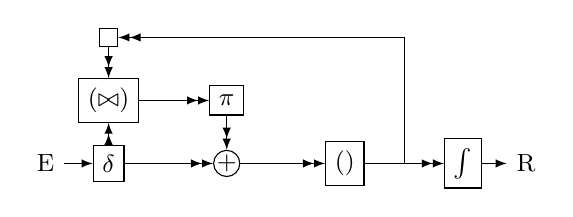
\begin{tikzpicture}[>=latex, node distance=1.5cm]
  \node[] (Einput) {\code{E}};
  % generic part
  \node[block, right of=Einput, node distance=.8cm] (E) {$\delta$};

  % relational query
  \node[block, above of=E, node distance=.8cm] (j) {$\inc{(\lift{\bowtie})}$};
  \node[block, right of=j] (pj) {$\lift{\pi}$};
  \node[block, circle, below of=pj, node distance=.8cm, inner sep=0cm] (plus) {$+$};
  \node[block, right of=plus] (d) {$\inc{(\lift{\distinct})}$};
  \draw[->>] (E) -- (j);
  \draw[->>] (j) -- (pj);
  \draw[->>] (E) -- (plus);
  \draw[->>] (pj) -- (plus);
  \draw[->>] (plus) -- (d);

  % generic part
  \node[block, right of=d] (S) {$\int$};
  \node[right of=S, node distance=.8cm] (output)  {\code{R}};
  \draw[->] (Einput) -- (E);
  \draw[->>] (d) -- node (o) {} (S);
  \draw[->] (S) -- (output);
  \node[block, above of=j, node distance=.8cm] (z) {$\zm$};
  \draw[->>] (o.center) |- (z);
  \draw[->>] (z) -- (j);
\end{tikzpicture}

This circuit contains two lifted incremental operators; a join and a
distinct; these can be further expanded into simpler primitives as in
the final step in Section~\ref{sec:relational-example}.  This
implementation matches the efficiency of Datalog semi-naive evaluation
engines, but does not yet handle incremental updates.  These are the
subject of the next section.


\input{nested}
\input{extensions}
\section{Implementation}\label{sec:implementation}

\subsection{Formal verification}

We have formalized and verified all the definitions, lemmas,
propositions, theorems, and examples in this paper using the Lean theorem prover; we make
these proofs available at~\cite{dbsp-theory}.
% This amounted to roughly 5K lines of Lean code.
The formalization builds on mathlib~\cite{mathlib2020}, which provides
support for groups and functions with finite support (modeling
\zrs). We believe the simplicity of \dbsp enabled completing these
proofs in relatively few lines of Lean code (5K) and keeping a close
correspondence between the paper proofs in~\cite{tr} and Lean.

\subsection{The \dbsp Rust runtime}

We have built an implementation of \dbsp as part of an
open-source project with an MIT license:
\url{https://github.com/feldera/feldera}.
The implementation consists of a Rust library and a runtime.
The library provides APIs for basic algebraic data types:
such as groups, finite maps, \zr, indexed \zr.
A separate circuit construction API allows users to
create \dbsp circuits by placing operator nodes (corresponding to boxes in our diagrams)
and connecting them with streams, which correspond to the
arrows in our diagrams.  The library provides pre-built generic operators
for integration, differentiation, delay, nested integration and differentiation,
and a rich library of \zr basic incremental operators:
corresponding to plus, negation, grouping, joining, aggregation, $\distinct$,
flatmap, window aggregates, etc.

For iterative computations the library provides the $\delta_0$ operator and
an operator that approximates $\int$ by terminating iteration of
a loop at a user-specified condition (usually the condition is the
requirement for a zero to appear in a specified stream).
The low level library allows users to construct incremental
circuits manually by stitching together incremental versions of primitive operators.

The library supports data-parallel multicore evaluation of circuits
using a natural sharding strategy, and a variety of adapters for
external data sources (e.g., Kafka, CSV files, etc).  The library can
also spill internal operator state to persistent storage.  Benchmark
results (which are very promising) are available in the code
repository and will be discussed in future work.

\subsection{Parallelization and Scale-out}

\subsection{State management}

\textbf{Tradeoffs.}  Incremental computation is not free.  It is in
fact a trade-off between time and space.  In the cost analysis we have
to consider both the time and the space used by each operator.  While
many incremental database operations can be implemented using work
proportional to the size of the changes, and no storage overhead,
several classes of database operations, such as joins, ``distinct'',
and aggregates can be implemented efficiently only using additional
storage in the form of \emph{indexes}.  The size of these indexes is
proportional to the size of the total data in the database (and not
just to the size of the changes) --- and since some indexes are over
intermediate relations, they can even exceed the size of the original
database.  In \dbsp the indexes are represented by delay operators
$\zm$.  In fact, the delay operator (and its lifted variant
$\lift{\zm}$) are the only operators that maintains state.  This is
also the only state that needs to be persisted, checkpointed, or
migrated to make \dbsp computations fault-tolerant.

\dbsp is an ``eager'' or ``top-down'' execution model: it constantly
maintains the entire contents of any number of views, even if no one
really wants to inspect the views.  In contrast, ``lazy'' or
``bottom-up'' models only build part of the views when the views are
inspected.  Such models have the potential to be more efficient.
Eager models can be converted into lazy ones if something is known
about the class of operations that will be executed against the views.



TODO: the LSM data structure, storage organization

\subsubsection{Checkpointing and fault-tolerance}

\subsection{SQL compiler}

We have also built a SQL to \dbsp compiler, which translates standard
SQL queries into \dbsp circuits.  The compiler implements
Algorithm~\ref{algorithm-inc}, to generate a streaming version of any
SQL query.  The compiler is open-source
\url{https://github.com/feldera/feldera/sql-to-dbsp-compiler} with
an MIT license.  The compiler front-end parser and optimizer are based
on the Apache Calcite~\cite{begoli-icmd18} infrastructure.  The
project is mature enough to pass all 7 million SQL Logic
Tests~\cite{sqllogictest}.  The compiler handles all aspects of SQL,
including NULLs, ternary logic, grouping, aggregation, multiset
queries, etc.  Currently correlated sub-queries and outer joins are
essentially converted to equivalent relational plans using multiple
joins.

\subsection{Streaming SQL extensions}


\section{Related work}\label{sec:related}

Incremental view
maintenance~\cite{buneman-actd79,blakeley-sigmod86,gupta-sigmod93,chaudhuri-icde95,gupta-idb95,chirkova-book12}
is a much studied problem in databases.  A survey of results for
Datalog queries is present in~\cite{motik-ai19}.  The standard
approach is as follows: given a query $Q$, discover a ``delta query'',
a ``differential'' version $\Delta Q$ that satisfies the equation:
$Q(d+\Delta d)=Q(d)+\Delta Q(d,\Delta d)$, and which can be used to
compute the change for a new input reusing the previous output.
DBToaster introduced recursive recursive
IVM~\cite{ahmad-vldb09,koch-pods10}, where the incrementalization
process is repeated for the delta query.

\cite{bello-vldb98} describes an early implementation in Oracle~8,
which handles a limited set of queries.  Many custom algorithms were
published for various classes of queries:
e.g. \cite{griffin-sigmod98,larson-icde07} for various classes of
joins, \cite{koch-pods16} handles positive nested relational calculus,
\cite{gupta-infsys06} handles relational and aggregate operators,
\cite{kara-tds20} is optimized for triangle queries,
DYN~\cite{idris-sigmod17,idris-vldb18,idris-sigmod19} focuses on
acyclic conjunctive queries: instead of keeping the output view
materialized they build data structures that allow efficiently
querying the output views.  PAI maps~\cite{abeysinghe-sigmod22} are
specially designed for queries with correlated aggregations.
\cite{katsis-sigmod15} uses primary key information to compress the
representation of the deltas, and using an ``update'' operator that is
similar to our ``upsert'' operator.  AJU~\cite{wang-sigmod20} and
\cite{svingos-amd23} focuse use foreign key information to optimize
query plan generation.  These techniques are only sound in the absence
of deletions and updates; Feldera uses these optimizations as well.  .
Some algorithms apply to sets, some work for
multisets~\cite{griffin-sigmod95}.  Many of these formalisms look very
complicated because they deal with ``insertions'', ``deletions'', and
``update'' changes separately.  \zrs are a much more compact tool for
describing such algorithms.  In some sense the \dbsp theory, through
the chain rule, enables us to reuse all of these results: given a good
implementation strategy for a particular query plan it can be reused
as a subplan in any query which can be made to use that particular
plan.

\dbsp as described implies an ``eager'' execution model: it constantly
maintains the entire contents of any number of views, even if no one
really wants to inspect the views.  In contrast, ``lazy''
models~\cite{hanson-sigmod87} only build part of the views when the
views are inspected.  Such models have the potential to be more
efficient.  A simple way to implement a ``lazy'' model using \dbsp is
to essentially accumulate all input changes as \zrs and apply the
incremental algorithm only when the output view is queried.  In
between are ``snapshot'' views, which are updated
periodically~\cite{colby-sigmod97}.

\cite{bengoli-sigmod19} proposes using SQL to express both standard
database queries and streaming queries and provides an implementation
for RedShift.  While this is a very nice goal, the \dbsp theory allows
us to formally argue that there are many classes of queries that
cannot be expressed in SQL.  So the question becomes perhaps ``what
are the minimal changes that should be made to SQL to enable enabling
stream processing?''

\dbsp is a bottom-up system, which always produces eagerly the
\emph{changes} to the output views.  Instead of maintaining the output
view entirely, \dbsp proposes generating deltas as the output of the
computation (similar to the kSQL~\cite{jafarpour-edbt19} \texttt{EMIT
  CHANGES} queries).  The idea that both inputs and outputs to an IVM
system are streams of changes seems trivial, but this is key to the
symmetry of our solution: both in our definition of
IVM~(\ref{def:inc}), and the fundamental reason that the chain rule
exists --- the chain rule is the one that makes our structural
induction IVM algorithm possible.

Several IVM algorithms for Datalog-like languages use counting based
approaches~\cite{Dewan-iis92,motik-aaai15} that maintain the number of
derivations of each output fact: DRed~\cite{gupta-sigmod93} and its
variants~\cite{Ceri-VLDB91,Wolfson-sigmod91,Staudt-vldb96,Kotowski-rr11,Lu-sigmod95,Apt-sigmod87},
the backward-forward algorithm and
variants~\cite{motik-aaai15,Harrison-wdd92,motik-ai19}.  \dbsp is more
general, and our incrementalization algorithm handles arbitrary
recursive queries and generates more efficient plans for recursive
queries in the presence of arbitrary updates (especially deletions,
where competing approaches may over-delete).  Interestingly, the \zrs
weights in \dbsp are related to the counting-number-of-derivations
approaches, but our use of the $\distinct$ operator shows that precise
counting is not necessary.

Picallo et al.~\cite{picallo-scop19} provide a general solution to IVM
for rich languages.  \dbsp requires a group structure on the values
operated on; this assumption has two major practical benefits: it
simplifies the mathematics considerably (e.g., Picallo uses monoid
actions to model changes), and it provides a general, simple algorithm
(\ref{algorithm-inc}) for incrementalizing arbitrary programs.  The
downside of \dbsp is that one has to find a suitable group structure
(e.g., \zrs for sets) to ``embed'' the computation.  Picallo's notion
of ``derivative'' is not unique: they need creativity to choose the
right derivative definition, we need creativity to find the right
group structure.

Finding a suitable group structure has proven easy for relations
(both~\cite{koch-pods10} and~\cite{green-tcs11} use \zrs to uniformly
model data and insertions/deletions), but it is not obvious how to do
it for other data types, such as sorted collections, or tree-shaped
collections (e.g., XML or JSON documents)~\cite{foster-planx08}.  An
intriguing question is ``what other interesting group structures could
this be applied to besides \zrs?''  Papers such
as~\cite{nikolic-icmd18} explore other possibilities, such as matrix
algebra, linear ML models, or conjunctive queries.

\dbsp can also model window and stream database
queries~\cite{arasu-tr02,aurora} such as CQL queries.
Begoli~\cite{begoli-sigmod19} has proposed using SQL for streaming
computations.  While SQL can go a long way, the \dbsp theory shows
that there are computations that cannot be expressed in pure SQL (at
least not without changing the schema and structure of the data).  A
SQL query is a function of the state of the database; in other words,
a SQL query cannot provide different results based on the order of
insertions of tuples in a table.  Streaming systems however can.  So
the question becomes not whether SQL is suitable for stream
processing, but rather, how can SQL be modified in minimal way to
cover many important use cases that arise in the context of streaming
systems.

\cite{bonifati-iclp2018} implemented a verified IVM algorithm for a
particular class of graph queries called Regular Datalog, with an
implementation machine-checked in the Coq proof assistant. Their focus
is on a particular algorithm and the approach does not consider other
SQL operators, general recursion, or custom operators (although it is
modular in the sense that it works on any query by incrementalizing it
recursively). Furthermore, for all queries a deletion in the input
change stream requires running the non-incremental query to recover.
We formally verify the theorems in our paper, which are much broader
in scope, but not our implementations.


\dbsp is also related to Differential Dataflow
(DD)~\cite{mcsherry-cidr13,murray-sosp13} and its theoretical
foundations~\cite{abadi-fossacs15} (and
recently~\cite{mcsherry-vldb20,chothia-vldb16}).  DD's computational
model is more powerful than \dbsp, since it allows time values to be
part of an arbitrary lattice.  In fact, DD is the only other framework
which we are aware of that can incrementalize recursive queries as
efficiently as \dbsp does.  In contrast, our model uses either
``linear'' times, or nested time dimensions via the modular lifting
transformer ($\lift{}$).  \dbsp can express both incremental and
non-incremental computations.  Most importantly, \dbsp comes with
Algorithm~\ref{algorithm-inc}, a syntax-directed translation that can
convert any expressible query into an incremental version --- in DD
users have to assemble incremental queries manually using incremental
operators.  (materialize.com offers a product that automates
incrementalization for SQL queries based on DD.  Differential
Datalog~\cite{ryzhyk-datalog19} does it for a Datalog dialect.)
Unlike DD, \dbsp is a modular theory, which easily accommodates the
addition of new operators: as long as we can express a new operator as
a \dbsp circuit, we can (1) define its incremental version, (2) apply
the incrementalization algorithm to obtain an efficient incremental
implementation, and (3) be confident that it composes with any other
operators.

\cite{akidau-amd23,akidau-debs24} describe the Snowflake incremental
and streaming capabilities.  In Showflake ``streams'' are database
table that store the history of changes to a table.  Dynamic tables
are views which are periodically refreshed, at user-specified
intervals.  These can be updated either incrementally or using batch
recomputation; the system chooses a stragegy based on the refres
period.  The views provide snapshot isolation, which is similar to the
DBSP consistency model.

The \dbsp model is simple enough so it can be implemented in a few
hundred lines of Python~\cite{dbsp-python}.

\section{Conclusions}\label{sec:conclusions}%\label{sec:ddlog}

\subsection{Adoption}

Traditional databases do not offer efficient IVM implementations for
arbitrary queries.  Databases could in principle be retrofitted to use
the algorithms in this paper, but the existing query engines are not
built around structures that can represent negative changes (like
\zrs), so this effort will require a significant redesign.

Moreover, we argue that databases should not only compute views
incrementally, but should use ``changes'' as the fundamental data
structure to communicate with their environment: a database service
should offer the following API: users register to receive
notifications for changes in one or more views.  Then, for any
transaction committed, each user receives a notification containing
the list of changes for the all the views they registered.  Databases
today do not have convenient mechanism for reporting changes to the
outside world.  In fact, entire industries have sprung up around the
concept of Change Data Capture~\cite{cdc}, which is building ad-hoc
solutions for extracting changes from databases, usually by inspecting
the write-ahead transaction log.

\subsection{Summary}

We have introduced \dbsp, a model of computation based on infinite
streams over commutative groups.  In this model streams are used for 3
purposes: (1) to model consecutive snapshots of a database, (2) to
model consecutive changes (deltas, or transactions) applied to a
database and changes of a maintained view, (3) to model consecutive
values of loop-carried variables in recursive computations.

We have defined an abstract notion of incremental computation over
streams, and defined the incrementalization operator $\inc{\cdot}$,
which transforms an \emph{arbitrary} stream computation $Q$ into its
incremental version $\inc{Q}$.  The incrementalization operator has
some very nice algebraic properties, which gave us a general algorithm
for incrementalizing many classes of complex queries, including
arbitrary recursive queries.

We believe that \dbsp can form a solid foundation for a theory and
practice of streaming incremental computation.


\bibliographystyle{abbrv}
\bibliography{main}

\end{document}
